% File: rl_as_stacked_mab.tex
% A single slide illustrating Reinforcement Learning as a sequence of Multi-Armed Bandit problems.
% To be included in a main Beamer presentation using % File: rl_as_stacked_mab.tex
% A single slide illustrating Reinforcement Learning as a sequence of Multi-Armed Bandit problems.
% To be included in a main Beamer presentation using % File: rl_as_stacked_mab.tex
% A single slide illustrating Reinforcement Learning as a sequence of Multi-Armed Bandit problems.
% To be included in a main Beamer presentation using % File: rl_as_stacked_mab.tex
% A single slide illustrating Reinforcement Learning as a sequence of Multi-Armed Bandit problems.
% To be included in a main Beamer presentation using \input{rl_as_stacked_mab.tex}

\begin{frame}{Reinforcement Learning as Stacked Bandits}
\frametitle{From Bandits to Reinforcement Learning}

\begin{figure}[h]
    \centering
    \begin{tikzpicture}[
        % Style for nodes containing the octopus image
        bandit/.style={
            inner sep=0, % No extra padding around the image
        },
        % Style for the arrows connecting the bandit problems
        arrow/.style={
            -latex,      % Use LaTeX arrow tip
            thick,       % Make the line thick
            draw=blue!70, % A nice blue color
            shorten <=2pt, % Shorten start of arrow slightly
            shorten >=2pt, % Shorten end of arrow slightly
        },
        % Style for the labels on the arrows
        label/.style={
            midway,      % Position label in the middle of the path
            above,       % Position label above the path
            font=\small, % Use a small font size
            fill=white,  % Give it a white background to stand out
            inner sep=1pt, % A little padding around the text
        }
    ]
        % Node 1: The first bandit problem (state s_1)
        % This node appears on all slides of the frame.
        \node<1->[bandit] (img1) {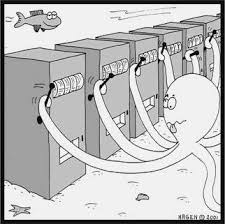
\includegraphics[width=0.2\textwidth]{octopus.png}};
        \node[below=1pt of img1] {$s_1$};

        % Node 2: The second bandit problem (state s_2)
        % This node appears from the second slide onwards.
        \node<2->[bandit, right=3cm of img1] (img2) {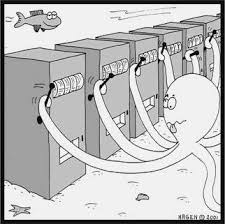
\includegraphics[width=0.2\textwidth]{octopus.png}};
        \node<2->[below=1pt of img2] {$s_2$};

        % Node 3: The third bandit problem (state s_3)
        % This node appears from the third slide onwards.
        \node<3->[bandit, right=3cm of img2] (img3) {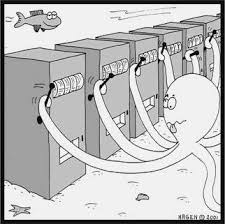
\includegraphics[width=0.2\textwidth]{octopus.png}};
        \node<3->[below=1pt of img3] {$s_3$};

        % Dots to indicate the sequence continues...
        % This appears from the fourth slide onwards.
        \node<4->[right=2cm of img3] (dots) {\Huge \dots};

        % Arrow 1: From s_1 to s_2
        % This appears on the second slide onwards.
        \draw<2->[arrow] (img1) -- (img2) node[label] {action $a_1$, get reward $r_1$};

        % Arrow 2: From s_2 to s_3
        % This appears on the third slide onwards.
        \draw<3->[arrow] (img2) -- (img3) node[label] {action $a_2$, get reward $r_2$};

    \end{tikzpicture}
    \caption{In RL, the action chosen in the current state (a bandit problem) determines the next state (a new bandit problem).}
\end{figure}

\end{frame}

\begin{frame}{Reinforcement Learning as Stacked Bandits}
\frametitle{From Bandits to Reinforcement Learning}

\begin{figure}[h]
    \centering
    \begin{tikzpicture}[
        % Style for nodes containing the octopus image
        bandit/.style={
            inner sep=0, % No extra padding around the image
        },
        % Style for the arrows connecting the bandit problems
        arrow/.style={
            -latex,      % Use LaTeX arrow tip
            thick,       % Make the line thick
            draw=blue!70, % A nice blue color
            shorten <=2pt, % Shorten start of arrow slightly
            shorten >=2pt, % Shorten end of arrow slightly
        },
        % Style for the labels on the arrows
        label/.style={
            midway,      % Position label in the middle of the path
            above,       % Position label above the path
            font=\small, % Use a small font size
            fill=white,  % Give it a white background to stand out
            inner sep=1pt, % A little padding around the text
        }
    ]
        % Node 1: The first bandit problem (state s_1)
        % This node appears on all slides of the frame.
        \node<1->[bandit] (img1) {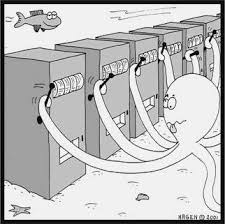
\includegraphics[width=0.2\textwidth]{octopus.png}};
        \node[below=1pt of img1] {$s_1$};

        % Node 2: The second bandit problem (state s_2)
        % This node appears from the second slide onwards.
        \node<2->[bandit, right=3cm of img1] (img2) {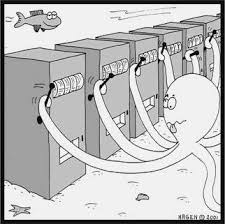
\includegraphics[width=0.2\textwidth]{octopus.png}};
        \node<2->[below=1pt of img2] {$s_2$};

        % Node 3: The third bandit problem (state s_3)
        % This node appears from the third slide onwards.
        \node<3->[bandit, right=3cm of img2] (img3) {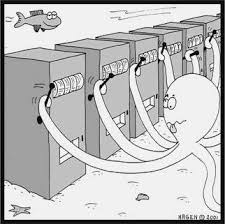
\includegraphics[width=0.2\textwidth]{octopus.png}};
        \node<3->[below=1pt of img3] {$s_3$};

        % Dots to indicate the sequence continues...
        % This appears from the fourth slide onwards.
        \node<4->[right=2cm of img3] (dots) {\Huge \dots};

        % Arrow 1: From s_1 to s_2
        % This appears on the second slide onwards.
        \draw<2->[arrow] (img1) -- (img2) node[label] {action $a_1$, get reward $r_1$};

        % Arrow 2: From s_2 to s_3
        % This appears on the third slide onwards.
        \draw<3->[arrow] (img2) -- (img3) node[label] {action $a_2$, get reward $r_2$};

    \end{tikzpicture}
    \caption{In RL, the action chosen in the current state (a bandit problem) determines the next state (a new bandit problem).}
\end{figure}

\end{frame}

\begin{frame}{Reinforcement Learning as Stacked Bandits}
\frametitle{From Bandits to Reinforcement Learning}

\begin{figure}[h]
    \centering
    \begin{tikzpicture}[
        % Style for nodes containing the octopus image
        bandit/.style={
            inner sep=0, % No extra padding around the image
        },
        % Style for the arrows connecting the bandit problems
        arrow/.style={
            -latex,      % Use LaTeX arrow tip
            thick,       % Make the line thick
            draw=blue!70, % A nice blue color
            shorten <=2pt, % Shorten start of arrow slightly
            shorten >=2pt, % Shorten end of arrow slightly
        },
        % Style for the labels on the arrows
        label/.style={
            midway,      % Position label in the middle of the path
            above,       % Position label above the path
            font=\small, % Use a small font size
            fill=white,  % Give it a white background to stand out
            inner sep=1pt, % A little padding around the text
        }
    ]
        % Node 1: The first bandit problem (state s_1)
        % This node appears on all slides of the frame.
        \node<1->[bandit] (img1) {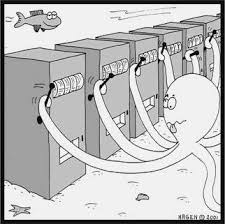
\includegraphics[width=0.2\textwidth]{octopus.png}};
        \node[below=1pt of img1] {$s_1$};

        % Node 2: The second bandit problem (state s_2)
        % This node appears from the second slide onwards.
        \node<2->[bandit, right=3cm of img1] (img2) {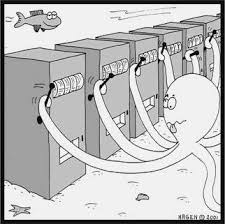
\includegraphics[width=0.2\textwidth]{octopus.png}};
        \node<2->[below=1pt of img2] {$s_2$};

        % Node 3: The third bandit problem (state s_3)
        % This node appears from the third slide onwards.
        \node<3->[bandit, right=3cm of img2] (img3) {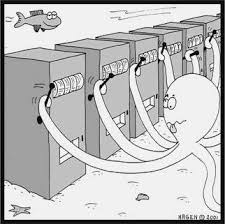
\includegraphics[width=0.2\textwidth]{octopus.png}};
        \node<3->[below=1pt of img3] {$s_3$};

        % Dots to indicate the sequence continues...
        % This appears from the fourth slide onwards.
        \node<4->[right=2cm of img3] (dots) {\Huge \dots};

        % Arrow 1: From s_1 to s_2
        % This appears on the second slide onwards.
        \draw<2->[arrow] (img1) -- (img2) node[label] {action $a_1$, get reward $r_1$};

        % Arrow 2: From s_2 to s_3
        % This appears on the third slide onwards.
        \draw<3->[arrow] (img2) -- (img3) node[label] {action $a_2$, get reward $r_2$};

    \end{tikzpicture}
    \caption{In RL, the action chosen in the current state (a bandit problem) determines the next state (a new bandit problem).}
\end{figure}

\end{frame}

\begin{frame}{Reinforcement Learning as Stacked Bandits}
\frametitle{From Bandits to Reinforcement Learning}

\begin{figure}[h]
    \centering
    \begin{tikzpicture}[
        % Style for nodes containing the octopus image
        bandit/.style={
            inner sep=0, % No extra padding around the image
        },
        % Style for the arrows connecting the bandit problems
        arrow/.style={
            -latex,      % Use LaTeX arrow tip
            thick,       % Make the line thick
            draw=blue!70, % A nice blue color
            shorten <=2pt, % Shorten start of arrow slightly
            shorten >=2pt, % Shorten end of arrow slightly
        },
        % Style for the labels on the arrows
        label/.style={
            midway,      % Position label in the middle of the path
            above,       % Position label above the path
            font=\small, % Use a small font size
            fill=white,  % Give it a white background to stand out
            inner sep=1pt, % A little padding around the text
        }
    ]
        % Node 1: The first bandit problem (state s_1)
        % This node appears on all slides of the frame.
        \node<1->[bandit] (img1) {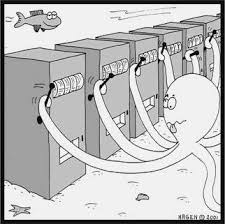
\includegraphics[width=0.2\textwidth]{octopus.png}};
        \node[below=1pt of img1] {$s_1$};

        % Node 2: The second bandit problem (state s_2)
        % This node appears from the second slide onwards.
        \node<2->[bandit, right=3cm of img1] (img2) {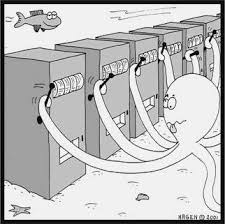
\includegraphics[width=0.2\textwidth]{octopus.png}};
        \node<2->[below=1pt of img2] {$s_2$};

        % Node 3: The third bandit problem (state s_3)
        % This node appears from the third slide onwards.
        \node<3->[bandit, right=3cm of img2] (img3) {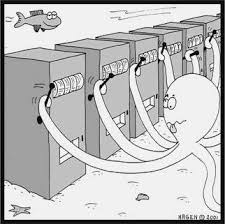
\includegraphics[width=0.2\textwidth]{octopus.png}};
        \node<3->[below=1pt of img3] {$s_3$};

        % Dots to indicate the sequence continues...
        % This appears from the fourth slide onwards.
        \node<4->[right=2cm of img3] (dots) {\Huge \dots};

        % Arrow 1: From s_1 to s_2
        % This appears on the second slide onwards.
        \draw<2->[arrow] (img1) -- (img2) node[label] {action $a_1$, get reward $r_1$};

        % Arrow 2: From s_2 to s_3
        % This appears on the third slide onwards.
        \draw<3->[arrow] (img2) -- (img3) node[label] {action $a_2$, get reward $r_2$};

    \end{tikzpicture}
    \caption{In RL, the action chosen in the current state (a bandit problem) determines the next state (a new bandit problem).}
\end{figure}

\end{frame}